% answers.tex —— 2017 年·天津卷·理科 · 参考答案与详细解析片段
% 由 tools/generate_projects.py 依来源总账自 2017/2017_数学真题_天津理_试题.md + 2017/2017_数学真题_天津理_解析正文.md + 2017/2017_数学真题_天津理_答案要点.md 生成，勿手改（改源 MD 后重跑）


\begin{gknotice}
\textbf{解析归属}：固定来源仅含题面。以下由本库独立推导并经异人盲核，非官方解析；结论等级至多为 D。
第 17 题第（3）问保留 U：按题面线角条件有两个合法的 $AH$ 值；第 19 题图示未规定点 $P,Q$ 的上下次序。问题登记详见项目问题总账。
\end{gknotice}

\begin{answer}
\gksolhead{1}{}

\textbf{题目}：

设集合 $A=\{1,2,4,6\}$，$B=\{2,4\}$，$C=\{x\in\mathbb R\mid -1\leqslant x\leqslant5\}$，则 $(A\cup B)\cap C=$（　）

\begin{itemize}
\item (A) $\{2\}$
\item (B) $\{1,2,4\}$
\item (C) $\{1,2,4,5\}$
\item (D) $\{x\in\mathbb R\mid -1\leqslant x\leqslant5\}$
\end{itemize}

\Needspace{4\baselineskip}
\textbf{解析}

$A\cup B=\{1,2,4,6\}$，与区间 $[-1,5]$ 相交得 $\{1,2,4\}$。

\gkanswer{答案：B}

\end{answer}
\begin{answer}
\gksolhead{2}{}

\textbf{题目}：

\Needspace{5\baselineskip}
设变量 $x,y$ 满足约束条件
\nopagebreak[4]
\[
\begin{cases}
2x+y\geqslant0,\\
x+2y-2\geqslant0,\\
x\leqslant0,\\
y\leqslant3,
\end{cases}
\]
则目标函数 $z=x+y$ 的最大值为（　）

\begin{itemize}
\item (A) $\dfrac23$
\item (B) $1$
\item (C) $\dfrac32$
\item (D) $3$
\end{itemize}

\Needspace{4\baselineskip}
\textbf{解析}

由 $x\leqslant0$、$y\leqslant3$ 及目标函数 $x+y$，有 $z\leqslant3$。点 $(0,3)$ 满足另外两个约束，故最大值为 $3$。

\gkanswer{答案：D，最大值 $3$}

\end{answer}
\begin{answer}
\gksolhead{3}{}

\textbf{题目}：

阅读程序框图，运行相应的程序，若输入 $N$ 的值为 $24$，则输出 $N$ 的值为（　）
\nopagebreak[4]
\begin{center}\begin{tikzpicture}[>=stealth,thick,
  term/.style={draw,rounded corners=3pt,minimum width=21mm,minimum height=7mm},
  proc/.style={draw,minimum width=28mm,minimum height=8mm,align=center},
  test/.style={draw,diamond,aspect=2.35,inner sep=1pt,align=center},
  io/.style={draw,trapezium,trapezium left angle=70,trapezium right angle=110,
    minimum width=25mm,minimum height=8mm,align=center}]
  \node[term] (start) at (0,0) {开始};
  \node[io] (input) at (0,-1.15) {输入 $N$};
  \node[test] (div) at (0,-2.65) {$N$ 能被 $3$ 整除？};
  \node[proc] (divide) at (-2.9,-4.5) {$N=N/3$};
  \node[proc] (minus) at (2.9,-4.5) {$N=N-1$};
  \node[test] (small) at (0,-5.55) {$N\leq 3$？};
  \node[io] (output) at (0,-7.05) {输出 $N$};
  \node[term] (stop) at (0,-8.2) {结束};
  \draw[->] (start)--(input);
  \draw[->] (input)--(div);
  \draw[->] (div.south)--(0,-3.8)--(-2.9,-3.8)--(divide.north);
  \node at (.38,-3.55) {是};
  \draw[->] (div.east)--node[above]{否} ++(1.0,0)|-(minus.north);
  \draw[->] (divide.south)|-(small.west);
  \draw[->] (minus.south)|-(small.east);
  \draw[->] (small.south)--node[right]{是}(output.north);
  \draw[->] (output)--(stop);
  \draw[->] (small.west)--(-3.8,-5.55)--node[pos=.78,left]{否}(-3.8,-2.65)--(div.west);
\end{tikzpicture}
\end{center}
\nopagebreak[4]
\begin{itemize}
\item (A) $0$
\item (B) $1$
\item (C) $2$
\item (D) $3$
\end{itemize}

\Needspace{4\baselineskip}
\textbf{解析}

按框图从 $N=24$ 开始：$24\to8\to7\to6\to2$，此时 $N\leqslant3$，输出 $2$。

\gkanswer{答案：C，输出 $2$}

\end{answer}
\begin{answer}
\gksolhead{4}{}

\textbf{题目}：

设 $\theta\in\mathbb R$，则“$\left|\theta-\dfrac\pi{12}\right|<\dfrac\pi{12}$”是“$\sin\theta<\dfrac12$”的（　）

\begin{itemize}
\item (A) 充分而不必要条件
\item (B) 必要而不充分条件
\item (C) 充要条件
\item (D) 既不充分也不必要条件
\end{itemize}

\Needspace{4\baselineskip}
\textbf{解析}

$\left|\theta-\dfrac\pi{12}\right|<\dfrac\pi{12}$ 等价于 $0<\theta<\dfrac\pi6$，因而 $\sin\theta<\dfrac12$，是充分条件。反例 $\theta=-\dfrac\pi2$ 满足 $\sin\theta<\dfrac12$，但不满足前件，故非必要。

\gkanswer{答案：A}

\end{answer}
\begin{answer}
\gksolhead{5}{}

\textbf{题目}：

已知双曲线 $\dfrac{x^2}{a^2}-\dfrac{y^2}{b^2}=1\ (a>0,b>0)$ 的左焦点为 $F$，离心率为 $\sqrt2$。若经过 $F$ 和 $P(0,4)$ 两点的直线平行于双曲线的一条渐近线，则双曲线的方程为（　）

\begin{itemize}
\item (A) $\dfrac{x^2}{4}-\dfrac{y^2}{4}=1$
\item (B) $\dfrac{x^2}{8}-\dfrac{y^2}{8}=1$
\item (C) $\dfrac{x^2}{4}-\dfrac{y^2}{8}=1$
\item (D) $\dfrac{x^2}{8}-\dfrac{y^2}{4}=1$
\end{itemize}

\Needspace{4\baselineskip}
\textbf{解析}

设焦距为 $c$。离心率 $\sqrt2$ 给出 $c=\sqrt2a$，于是 $b^2=c^2-a^2=a^2$，渐近线斜率为 $\pm1$。直线 $FP$ 的斜率为 $4/c$；与渐近线平行给出 $c=4$，从而 $a^2=b^2=8$。

\gkanswer{答案：B}

\end{answer}
\begin{answer}
\gksolhead{6}{}

\textbf{题目}：

已知奇函数 $f(x)$ 在 $\mathbb R$ 上是增函数，$g(x)=xf(x)$。若 $a=g(-\log_2 5.1)$，$b=g(2^{0.8})$，$c=g(3)$，则 $a,b,c$ 的大小关系为（　）

\begin{itemize}
\item (A) $a<b<c$
\item (B) $c<b<a$
\item (C) $b<a<c$
\item (D) $b<c<a$
\end{itemize}

\Needspace{4\baselineskip}
\textbf{解析}

\Needspace{5\baselineskip}
奇函数且严格递增意味着 $f(x)>0$（$x>0$）。故 $g(x)=xf(x)$ 在正半轴严格递增，并且 $g(-x)=g(x)$。比较
\nopagebreak[4]
\[
2^{0.8}<\log_2 5.1<3
\]
（例如 $2^{0.8}<2$，而 $5.1>4$ 给出 $\log_2 5.1>2$，且 $5.1<8$），得 $b<a<c$。

\gkanswer{答案：C}

\end{answer}
\begin{answer}
\gksolhead{7}{}

\textbf{题目}：

设函数 $f(x)=2\sin(\omega x+\varphi)$，$x\in\mathbb R$，其中 $\omega>0$，$|\varphi|<\pi$。若 $f\left(\dfrac{5\pi}{8}\right)=2$，$f\left(\dfrac{11\pi}{8}\right)=0$，且 $f(x)$ 的最小正周期大于 $2\pi$，则（　）

\begin{itemize}
\item (A) $\omega=\dfrac23,\ \varphi=\dfrac\pi{12}$
\item (B) $\omega=\dfrac23,\ \varphi=-\dfrac{11\pi}{12}$
\item (C) $\omega=\dfrac13,\ \varphi=-\dfrac{11\pi}{24}$
\item (D) $\omega=\dfrac13,\ \varphi=\dfrac{7\pi}{24}$
\end{itemize}

\Needspace{4\baselineskip}
\textbf{解析}

周期大于 $2\pi$ 意味着 $0<\omega<1$。第一条件要求 $\frac{5\pi\omega}{8}+\varphi=\frac\pi2+2k\pi$，第二条件要求 $\frac{11\pi\omega}{8}+\varphi=n\pi$。相减得 $\frac{3\omega}{4}=n-2k-\frac12$。结合 $0<\frac{3\omega}{4}<\frac34$，只能有 $\omega=\frac23$；代回并用 $|\varphi|<\pi$ 得 $\varphi=\frac\pi{12}$。

\gkanswer{答案：A}

\end{answer}
\begin{answer}
\gksolhead{8}{}

\textbf{题目}：

\Needspace{5\baselineskip}
已知函数
\nopagebreak[4]
\[
f(x)=
\begin{cases}
x^2-x+3,&x\leqslant1,\\
x+\dfrac2x,&x>1,
\end{cases}
\]
设 $a\in\mathbb R$，若关于 $x$ 的不等式 $f(x)\geqslant\left|\dfrac x2+a\right|$ 在 $\mathbb R$ 上恒成立，则 $a$ 的取值范围是（　）

\begin{itemize}
\item (A) $\left[-\dfrac{47}{16},2\right]$
\item (B) $\left[-\dfrac{47}{16},\dfrac{39}{16}\right]$
\item (C) $[-2\sqrt3,2]$
\item (D) $\left[-2\sqrt3,\dfrac{39}{16}\right]$
\end{itemize}

\Needspace{4\baselineskip}
\textbf{解析}

\Needspace{5\baselineskip}
不等式 $f(x)\geqslant|x/2+a|$ 对所有 $x$ 成立，当且仅当
\nopagebreak[4]
\[
-f(x)-\frac x2\leqslant a\leqslant f(x)-\frac x2\quad(\forall x).
\]
因此下界为 $-\inf(f(x)+x/2)$，上界为 $\inf(f(x)-x/2)$。在 $x\leqslant1$ 时，$f+x/2=x^2-x/2+3$ 于 $x=1/4$ 取最小值 $47/16$；$f-x/2=x^2-3x/2+3$ 于 $x=3/4$ 取最小值 $39/16$。在 $x>1$ 时，两式分别为 $3x/2+2/x$（最小值 $2\sqrt3>47/16$）和 $x/2+2/x$（最小值 $2<39/16$）。所以 $a\in[-47/16,2]$。

\gkanswer{答案：A，$[-47/16,2]$}

\end{answer}
\gkpart{二、填空题}

\begin{answer}
\gksolhead{9}{}

\textbf{题目}：

已知 $a\in\mathbb R$，$i$ 为虚数单位，若 $\dfrac{a-i}{2+i}$ 为实数，则 $a$ 的值为\gkblank{}。

\Needspace{4\baselineskip}
\textbf{解析}

\nopagebreak[4]
\[
\frac{a-i}{2+i}=\frac{(a-i)(2-i)}5=\frac{2a-1}{5}-\frac{a+2}{5}i.
\]
虚部为零得 $a=-2$。

\gkanswer{答案：$-2$}

\end{answer}
\begin{answer}
\gksolhead{10}{}

\textbf{题目}：

已知一个正方体的所有顶点在一个球面上，若这个正方体的表面积为 $18$，则这个球的体积为\gkblank{}。

\Needspace{4\baselineskip}
\textbf{解析}

设棱长为 $s$，则 $6s^2=18$，所以 $s=\sqrt3$。外接球半径为正方体体对角线的一半，即 $r=\sqrt3s/2=3/2$，故体积 $\frac43\pi r^3=9\pi/2$。

\gkanswer{答案：$9\pi/2$}

\end{answer}
\begin{answer}
\gksolhead{11}{}

\textbf{题目}：

在极坐标系中，直线 $4\rho\cos\left(\theta-\dfrac\pi6\right)+1=0$ 与圆 $\rho=2\sin\theta$ 的公共点的个数为\gkblank{}。

\Needspace{4\baselineskip}
\textbf{解析}

取 $x=\rho\cos\theta,y=\rho\sin\theta$。圆化为 $x^2+(y-1)^2=1$；直线化为 $2\sqrt3x+2y+1=0$。圆心 $(0,1)$ 到直线的距离为 $3/4<1$，故有两个交点。

\gkanswer{答案：$2$}

\end{answer}
\begin{answer}
\gksolhead{12}{}

\textbf{题目}：

若 $a,b\in\mathbb R$，$ab>0$，则 $\dfrac{a^4+4b^4+1}{ab}$ 的最小值为\gkblank{}。

\Needspace{4\baselineskip}
\textbf{解析}

令 $t=ab>0$。由 $a^4+4b^4\geqslant2\sqrt{4a^4b^4}=4t^2$，原式不小于 $4t+1/t\geqslant4$。等号可取到：$t=1/2$ 且 $a^4=4b^4$ 时有 $a^4=1/2,b^4=1/8$。最小值为 $4$。

\gkanswer{答案：最小值 $4$}

\end{answer}
\begin{answer}
\gksolhead{13}{}

\textbf{题目}：

在 $\triangle ABC$ 中，$\angle A=60^\circ$，$AB=3$，$AC=2$。若 $\overrightarrow{BD}=2\overrightarrow{DC}$，$\overrightarrow{AE}=\lambda\overrightarrow{AC}-\overrightarrow{AB}\ (\lambda\in\mathbb R)$，且 $\overrightarrow{AD}\cdot\overrightarrow{AE}=-4$，则 $\lambda$ 的值为\gkblank{}。

\Needspace{4\baselineskip}
\textbf{解析}

\Needspace{5\baselineskip}
令 $\mathbf u=\overrightarrow{AB}$、$\mathbf v=\overrightarrow{AC}$，则 $|\mathbf u|=3,|\mathbf v|=2,\mathbf u\cdot\mathbf v=3$。由 $\overrightarrow{BD}=2\overrightarrow{DC}$，得 $\overrightarrow{AD}=\frac13\mathbf u+\frac23\mathbf v$，而 $\overrightarrow{AE}=\lambda\mathbf v-\mathbf u$。故
\nopagebreak[4]
\[
\overrightarrow{AD}\cdot\overrightarrow{AE}
=\frac{11}{3}\lambda-5=-4,
\]
解得 $\lambda=3/11$。

\gkanswer{答案：$3/11$}

\end{answer}
\begin{answer}
\gksolhead{14}{}

\textbf{题目}：

用数字 $1,2,3,4,5,6,7,8,9$ 组成没有重复数字，且至多有一个数字是偶数的四位数，这样的四位数一共有\gkblank{}个。（用数字作答）

\Needspace{4\baselineskip}
\textbf{解析}

偶数字为 $2,4,6,8$ 共 4 个，奇数字为 5 个。全由奇数组成有 $P(5,4)=120$ 个；恰有一个偶数有 $4\cdot4\cdot P(5,3)=960$ 个。合计 $1080$。

\gkanswer{答案：$1080$}

\end{answer}
\gkpart{三、解答题}

\begin{answer}
\gksolhead{15}{}

\textbf{题目}：

在 $\triangle ABC$ 中，内角 $A,B,C$ 所对的边分别为 $a,b,c$。已知 $a>b$，$a=5$，$c=6$，$\sin B=\dfrac35$。

(1)   求 $b$ 和 $\sin A$ 的值；
(2)   求 $\sin\left(2A+\dfrac\pi4\right)$ 的值。

\Needspace{4\baselineskip}
\textbf{解析}

\gksubpart{(1)}

\Needspace{5\baselineskip}
$B$ 不可能为钝角（否则最大边应为 $b$，与 $a>b$ 矛盾），故 $\cos B=4/5$。由正弦定理，
\nopagebreak[4]
\[
\frac ca=\frac{\sin C}{\sin A}
=\cos B+\sin B\cot A,
\]
故 $6/5=4/5+(3/5)\cot A$，从而 $\cot A=2/3$、$\sin A=3/\sqrt{13}$。再由正弦定理得 $b=a\sin B/\sin A=\sqrt{13}$。

\gksubpart{(2)}

\Needspace{5\baselineskip}
又 $\sin2A=12/13$、$\cos2A=-5/13$，所以
\nopagebreak[4]
\[
\sin\left(2A+\frac\pi4\right)
=\frac{\sqrt2}{2}(\sin2A+\cos2A)
=\frac{7\sqrt2}{26}.
\]

\gkanswer{答案（1）：$b=\sqrt{13}$，$\sin A=3/\sqrt{13}$}

\gkanswer{答案（2）：$\sin(2A+\pi/4)=7\sqrt2/26$}

\end{answer}
\begin{answer}
\gksolhead{16}{}

\textbf{题目}：

从甲地到乙地要经过 3 个丁字路口，设各路口信号灯工作相互独立，且在各路口遇到红灯的概率分别为 $\dfrac12,\dfrac13,\dfrac14$。

(1)   设 $X$ 表示一辆车从甲地到乙地遇到红灯的个数，求随机变量 $X$ 的分布列和数学期望；
(2)   若有 2 辆车独立地从甲地到乙地，求这 2 辆车共遇到 1 个红灯的概率。

\Needspace{4\baselineskip}
\textbf{解析}

\gksubpart{(1)}

\Needspace{5\baselineskip}
记各路口遇红灯为独立 Bernoulli 事件，概率依次为 $1/2,1/3,1/4$。则
\nopagebreak[4]
\[
\begin{aligned}
P(X=0)&=\frac12\frac23\frac34=\frac14,\\
P(X=1)&=\frac12\frac23\frac34+\frac12\frac13\frac34+\frac12\frac23\frac14=\frac{11}{24},\\
P(X=3)&=\frac12\frac13\frac14=\frac1{24},\\
P(X=2)&=1-P(X=0)-P(X=1)-P(X=3)=\frac14.
\end{aligned}
\]
分布列为 $X=0,1,2,3$ 对应概率 $\frac14,\frac{11}{24},\frac14,\frac1{24}$；$E(X)=1/2+1/3+1/4=13/12$。

\gksubpart{(2)}

\Needspace{5\baselineskip}
两辆车的六个路口遭遇独立，总红灯数恰为 1 的概率为
\nopagebreak[4]
\[
2P(X=1)P(X=0)=2\cdot\frac{11}{24}\cdot\frac14=\frac{11}{48}.
\]

\gkanswer{答案（1）：$P(X=0,1,2,3)=(1/4,11/24,1/4,1/24)$，$E(X)=13/12$}

\gkanswer{答案（2）：$11/48$}

\end{answer}
\begin{answer}
\gksolhead{17}{}

\textbf{题目}：

如图，在三棱锥 $P-ABC$ 中，$PA\perp$ 底面 $ABC$，$\angle BAC=90^\circ$。点 $D,E,N$ 分别为棱 $PA,PC,BC$ 的中点，$M$ 是线段 $AD$ 的中点，$PA=AC=4$，$AB=2$。
\nopagebreak[4]
\begin{center}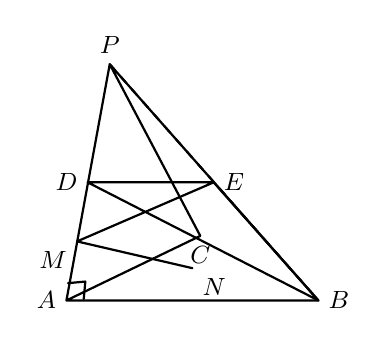
\begin{tikzpicture}[thick,line cap=round,line join=round,
  every node/.style={font=\small}]
  \coordinate (P) at (0,3.0);
  \coordinate (A) at (-.55,0);
  \coordinate (B) at (2.65,0);
  \coordinate (C) at (1.15,.82);
  \coordinate (D) at (-.28,1.5);
  \coordinate (E) at (1.32,1.5);
  \coordinate (N) at (1.05,.41);
  \coordinate (M) at (-.415,.75);
  % Outer pyramid and source-visible internal segments. The right-angle mark
  % is at A, as printed; no unlabelled construction point is added.
  \draw (P)--(A)--(B)--(P) (A)--(C) (P)--(C);
  \draw (B)--(D) (D)--(E) (B)--(E) (E)--(M) (M)--(N);
  \draw[dashed] (P)--(B);
  \draw (A) ++(.22,.02)--++(.02,.22)--++(-.22,-.02);
  \node[above] at (P) {$P$};
  \node[left] at (A) {$A$};
  \node[right] at (B) {$B$};
  \node[below] at (C) {$C$};
  \node[left] at (D) {$D$};
  \node[right] at (E) {$E$};
  \node[below left] at (M) {$M$};
  \node[below right] at (N) {$N$};
\end{tikzpicture}
\end{center}
\nopagebreak[4]
(1)   求证：$MN\parallel$ 平面 $BDE$；
(2)   求二面角 $C-EM-N$ 的正弦值；
(3)   已知点 $H$ 在棱 $PA$ 上，且直线 $NH$ 与直线 $BE$ 所成角的余弦值为 $\dfrac{\sqrt7}{21}$，求线段 $AH$ 的长。

\Needspace{4\baselineskip}
\textbf{解析}

\textbf{结论（U）}：题面条件未给出唯一的 $AH$ 值；推导如下。

取 $A=(0,0,0),B=(0,2,0),C=(4,0,0),P=(0,0,4)$，满足题给长度、直角及垂直关系。于是 $D=(0,0,2),E=(2,0,2),N=(2,1,0),M=(0,0,1)$。

\gksubpart{(1) 平面 $BDE$ 的方程为 $y+z=2$，法向量可取 $(0,1,1)$。$\overrightarrow{MN}=(2,1,-1)$ 与法向量点积为 $0$，且 $M$ 不在平面 $BDE$ 上，故 $MN\parallel$ 平面 $BDE$。}
\gksubpart{(2) 平面 $CEM$ 是 $y=0$，法向量可取 $(0,1,0)$。平面 $EMN$ 的法向量可取 $(1,-4,-2)$，模长为 $\sqrt{21}$。两平面夹角的正弦为 $\sqrt{1-(4/\sqrt{21})^2}=\sqrt{5/21}$。}
\gksubpart{(3) 令 $H=(0,0,h)$，$0\leqslant h\leqslant4$。则 $|NH|=\sqrt{h^2+5}$、$|BE|=2\sqrt3$，并且 $|\overrightarrow{NH}\cdot\overrightarrow{BE}|=|2(h-1)|$。按非定向直线夹角，条件等价于}
\nopagebreak[4]
\[
   \frac{|h-1|}{\sqrt{3(h^2+5)}}=\frac{\sqrt7}{21},
\]
   即 $10h^2-21h+8=0$，给出 $AH=h=1/2$ 或 $8/5$。两者均在棱 $PA$ 上且满足线角条件，故题面字面条件未确定唯一长度；保留为 U，待异人核查，不能任选其一。

\gkanswer{答案（1）：$MN\parallel$ 平面 $BDE$}

\gkanswer{答案（2）：两平面夹角的正弦为 $\sqrt{5/21}$}

\gkanswer{答案（3）：$AH=1/2$ 或 $8/5$}

\end{answer}
\begin{answer}
\gksolhead{18}{}

\textbf{题目}：

已知 $\{a_n\}$ 为等差数列，前 $n$ 项和为 $S_n\ (n\in\mathbb N^*)$，$\{b_n\}$ 是首项为 $2$ 的等比数列，且公比大于 $0$，$b_2+b_3=12$，$b_3=a_4-2a_1$，$S_{11}=11b_4$。

(1)   求 $\{a_n\}$ 和 $\{b_n\}$ 的通项公式；
(2)   求数列 $\{a_{2n}b_{2n-1}\}$ 的前 $n$ 项和 $\ (n\in\mathbb N^*)$。

\Needspace{4\baselineskip}
\textbf{解析}

\gksubpart{(1)}

设等比数列公比为 $q>0$。由 $b_2+b_3=12$ 得 $2q+2q^2=12$，故 $q=2$，即 $b_n=2^n$。设等差数列首项 $a_1$、公差 $d$。$b_3=a_4-2a_1$ 给出 $3d-a_1=8$；$S_{11}=11b_4$ 给出 $a_1+5d=16$。解得 $a_1=1,d=3$，所以 $a_n=3n-2$。

\gksubpart{(2)}

\nopagebreak[4]
\[
a_{2n}b_{2n-1}=(6n-2)2^{2n-1}=(3n-1)4^n.
\]
\Needspace{5\baselineskip}
故前 $n$ 项和
\nopagebreak[4]
\[
\sum_{k=1}^n(3k-1)4^k=\frac{8+(3n-2)4^{n+1}}3.
\]

\gkanswer{答案（1）：$a_n=3n-2,b_n=2^n$}

\gkanswer{答案（2）：$\sum_{k=1}^n a_{2k}b_{2k-1}=[8+(3n-2)4^{n+1}]/3$}

\end{answer}
\begin{answer}
\gksolhead{19}{}

\textbf{题目}：

设椭圆 $\dfrac{x^2}{a^2}+\dfrac{y^2}{b^2}=1\ (a>b>0)$ 的左焦点为 $F$，右顶点为 $A$，离心率为 $\dfrac12$。已知 $A$ 是抛物线 $y^2=2px\ (p>0)$ 的焦点，$F$ 到抛物线的准线 $l$ 的距离为 $\dfrac12$。

(1)   求椭圆的方程和抛物线的方程；
(2)   设 $l$ 上两点 $P,Q$ 关于 $x$ 轴对称，直线 $AP$ 与椭圆相交于点 $B\ (B$ 异于 $A)$，直线 $BQ$ 与 $x$ 轴相交于点 $D$。若 $\triangle APD$ 的面积为 $\dfrac{\sqrt6}{2}$，求直线 $AP$ 的方程。

\Needspace{4\baselineskip}
\textbf{解析}

\gksubpart{(1)}

\Needspace{5\baselineskip}
设椭圆半长轴为 $a$、焦距为 $c$。$c/a=1/2$，而抛物线焦点为 $(p/2,0)=A=(a,0)$，故 $p=2a$，准线为 $x=-a$。左焦点为 $F=(-c,0)$，题设距离给出 $a-c=1/2$。联立 $c=a/2$ 得 $a=1,c=1/2,b^2=3/4,p=2$，故椭圆、抛物线分别为
\nopagebreak[4]
\[
x^2+\frac{y^2}{3/4}=1,\qquad y^2=4x.
\]

\gksubpart{(2)}

\Needspace{5\baselineskip}
设直线 $AP$ 的斜率为 $t$，则 $P=(-1,-2t)$。把 $y=t(x-1)$ 代入椭圆，除去 $A$ 对应根 $x=1$，得
\nopagebreak[4]
\[
B=\left(\frac{4t^2-3}{4t^2+3},-\frac{6t}{4t^2+3}\right).
\]
\Needspace{5\baselineskip}
由 $Q=(-1,2t)$，直线 $BQ$ 与 $x$ 轴的交点满足 $x_D=(2t^2-3)/(2t^2+3)$。于是
\nopagebreak[4]
\[
\operatorname{Area}(\triangle APD)=\frac12|t|\cdot2(1-x_D)=\frac{6|t|}{2t^2+3}.
\]
\Needspace{5\baselineskip}
令其为 $\sqrt6/2$，平方化简得 $(2t^2-3)^2=0$，故 $t=\pm\sqrt6/2$。直线为
\nopagebreak[4]
\[
y=\pm\frac{\sqrt6}{2}(x-1).
\]

\gkanswer{答案（1）：椭圆 $x^2+y^2/(3/4)=1$，抛物线 $y^2=4x$}

\gkanswer{答案（2）：直线 $y=\pm(\sqrt6/2)(x-1)$}

\end{answer}
\begin{answer}
\gksolhead{20}{}

\textbf{题目}：

\Needspace{5\baselineskip}
设 $a\in\mathbb Z$，已知定义在 $\mathbb R$ 上的函数
\nopagebreak[4]
\[
f(x)=2x^4+3x^3-3x^2-6x+a
\]
在区间 $(1,2)$ 内有一个零点 $x_0$，$g(x)$ 为 $f(x)$ 的导函数。

(1)   求 $g(x)$ 的单调区间；
(2)   设 $m\in[1,x_0)\cup(x_0,2]$，函数 $h(x)=g(x)(m-x_0)-f(m)$，求证：$h(m)h(x_0)<0$；
\Needspace{5\baselineskip}
(3)   求证：存在大于 $0$ 的常数 $A$，使得对于任意的正整数 $p,q$，且 $\dfrac pq\in[1,x_0)\cup(x_0,2]$，满足
\nopagebreak[4]
\[
\left|\frac pq-x_0\right|\geqslant\frac1{Aq^4}.
\]

\Needspace{4\baselineskip}
\textbf{解析}

\nopagebreak[4]
\[
g(x)=f'(x)=8x^3+9x^2-6x-6,\qquad g'(x)=24x^2+18x-6=6(4x-1)(x+1).
\]
\gksubpart{(1) 因此 $g$ 在 $(-\infty,-1)$、$(1/4,+\infty)$ 上递增，在 $(-1,1/4)$ 上递减。}
\gksubpart{(2) $g$ 在 $[1,2]$ 上严格递增。对 $m\ne x_0$，由拉格朗日中值定理，存在 $\xi$ 严格介于 $m,x_0$ 之间，使 $f(m)=f(m)-f(x_0)=g(\xi)(m-x_0)$。于是}
\nopagebreak[4]
\[
   h(m)=(m-x_0)(g(m)-g(\xi))>0,\qquad
   h(x_0)=(m-x_0)(g(x_0)-g(\xi))<0,
\]
   两种 $m<x_0$ 或 $m>x_0$ 情况均成立，故 $h(m)h(x_0)<0$。
\gksubpart{(3) 在 $[1,2]$ 上 $g$ 递增，$g(1)=5,g(2)=82$，故 $5\leqslant g(x)\leqslant82$。于是 $f$ 在 $[1,2]$ 严格递增，$x_0$ 是该闭区间内唯一零点；故对 $r=p/q\in[1,x_0)\cup(x_0,2]$ 有 $f(r)\ne0$。由于 $a\in\mathbb Z$，$q^4f(p/q)$ 为非零整数，因此 $|f(r)|\geqslant1/q^4$。再由中值定理，}
\nopagebreak[4]
\[
   \frac1{q^4}\leqslant|f(r)-f(x_0)|\leqslant82|r-x_0|,
\]
   取 $A=82>0$ 即得所证。

\gkanswer{答案（1）：$g$ 在 $(-\infty,-1)$、$(1/4,+\infty)$ 递增，在 $(-1,1/4)$ 递减}

\gkanswer{答案（2）：见解析版}

\gkanswer{答案（3）：见解析版}

\end{answer}